% !TeX root = ../main.tex
% Add the above to each chapter to make compiling the PDF easier in some editors.

\chapter{Introduction}\label{chapter:introduction}
Internet of Things (IoT) and data-driven techniques have revolutionized the industry. Cloud computing applications collect huge amounts of manufacturing data. As a key role in modern production facilities, predictive maintenance applications have fully embraced the Big Data revolution. By analyzing production and machine data future machine failures or working conditions can be predicted. This is especially helpful to reduce downtime of single machines or whole production lines \cite{ZHAO2019213}. 

\section{Problems of Predictive Maintenance for ball screw drives}
In a wide range of industrial machines ball screws are used, which translate rotatory into linear motion with high precision. During longtime use degradation lowers the stiffness within the ball screw components. This leads to an inaccurate position movement, which lowers the precision of the machine and therefore the production quality. In the worst case a whole machine failure may occur. For this reason, tracking the ball screw health condition is of great importance. In recent years, Predictive Maintenance research mainly focused on rolling bearings and gearboxes. Since industrial machines and components have different stages of operation, working cycles and installed sensors, requirements for the predictive maintenance algorithms vary. The transferability of predictive maintenance algorithms is difficult and does usually require adjustments. However, intelligent data-driven methods have been successfully developed. Unfortunately, a lot of these approaches assume monitoring data used for training and testing to be from the same data distribution. In reality this is not the case. Since the operating conditions, component degradation and machine settings may change, the fault characteristics of the machines do also change. Therefore, the fault diagnosis system which is trained on a limited amount of data can not generalize well on the testing data. Consequently, the diagnosis system might have an unsatisfactory performance in the real industrial scenario. This phenomena is called domain shift problem \cite{AZAMFAR2020103932}. 

\section{Traditional Predictive Maintenance Approaches}
As shown in fig. \ref{fig:hand_crafted_features_physical_models_deep_learning} health monitoring traditionally is restricted to physical-based or conventional data-driven approaches. The persistence of  physical laws to satisfactorily explain the underlying complexity of a machine sounds like a promising way for predictive maintenance. Besides that these models do not require any historical fault data \cite{AN201942}. Unfortunately in this scenario the physics we know needs to rely on data which is often perturbed. Not including these perturbations in the models reduces the performance. With the establishment of modern sensors, networks and computing systems data-driven approaches became into the focus of research. In conventional data-driven approaches traditional hand-crafted features are used to extract expressive information from the data in a first step. Subsequently a shallow classifier is responsible for an accurate prediction. Both just mentioned methods suffer from two problems. Firstly, in complex real-world problems establishing physical-based models or conventional hand-crafted features is quiet a laborious task and expect a lot of experience and human labor. Secondly, an in-line update with measured data is not possible. The physical-based models and hand-crafted features are restricted to the application of interest and its transferability is very limited. Therefore, the limited flexibility and effectiveness of the two traditional approaches is responsible for the growing interest in deep learning based Predictive Maintenance. Deep neural networks can capture relations within complex and high-dimensional data. By using multiple layers, neural networks can progressively extract higher-level features from the raw input. Due to the automatic learning of neural networks they can be adjusted quickly to different problems. Especially due to the increased amount of data, computation power and huge research the popularity of deep learning increased a lot.  \cite{ZHAO2019213} \cite{AZAMFAR2020103932}. 

\begin{figure}[htpb]
  \centering
  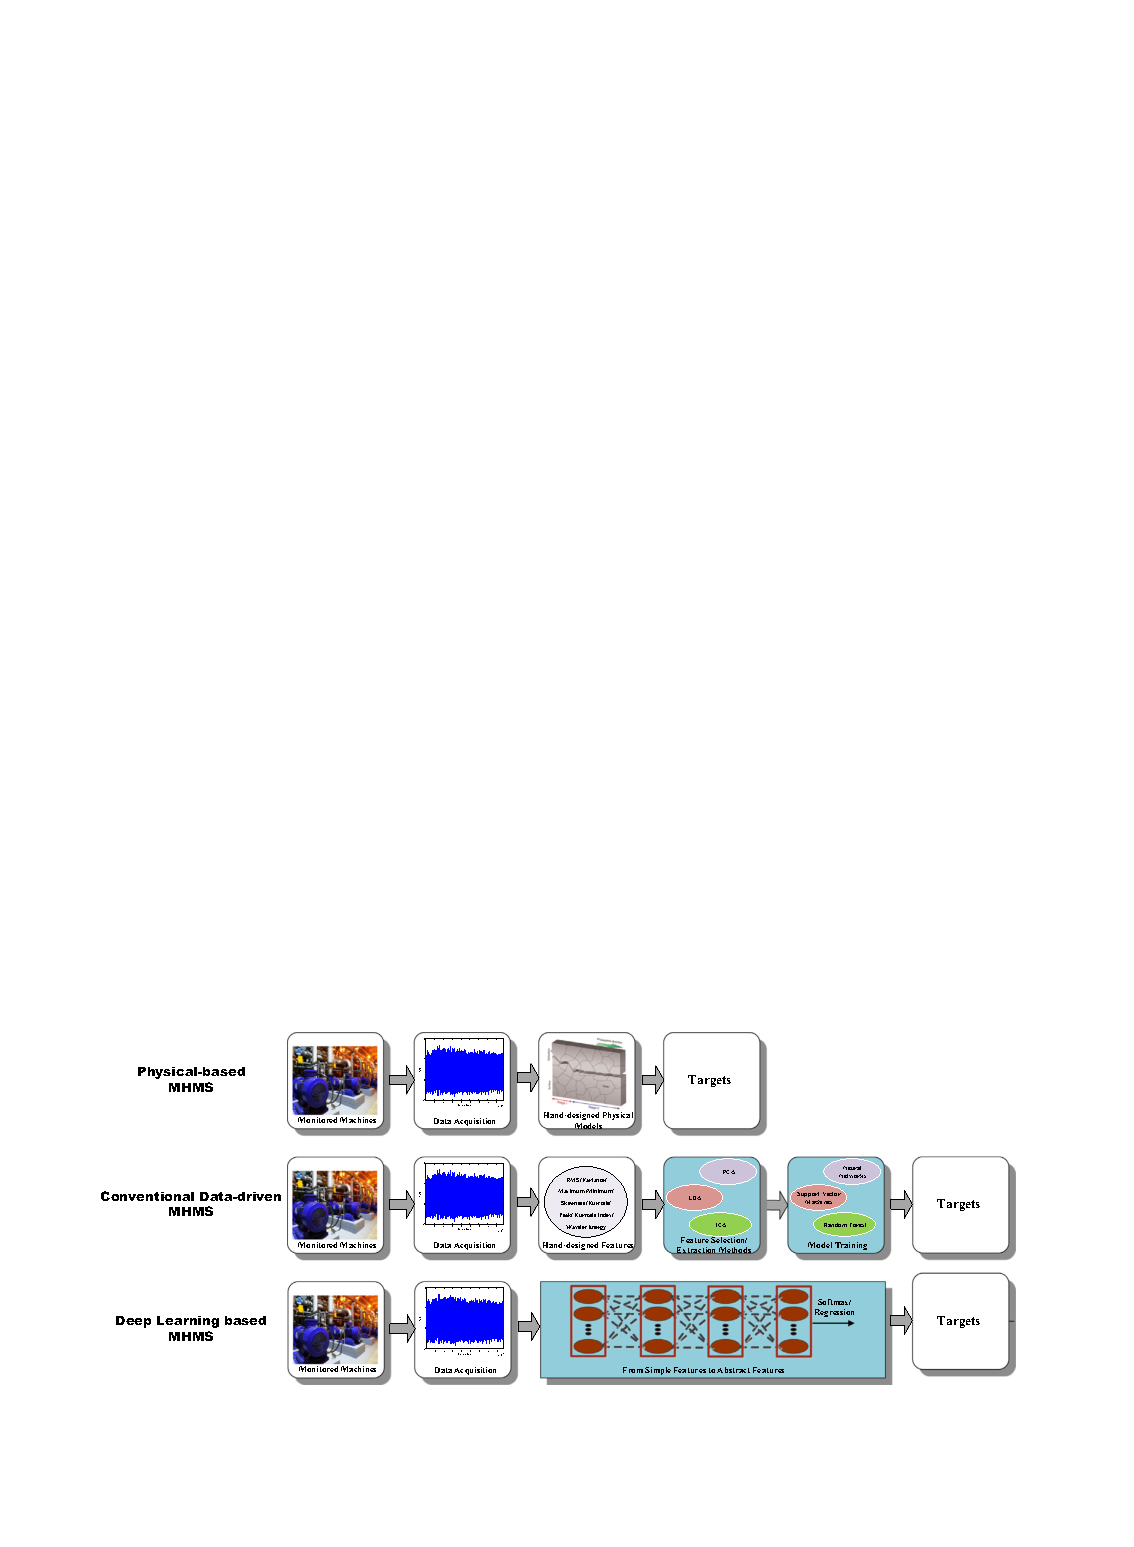
\includegraphics[width=1\textwidth]{hand_crafted_features_physical_models_deep_learning}
  \caption {Physical Models, Conventional Data-driven Models and Deep Learning Models for predictive maintenance \cite{ZHAO2019213}} \label{fig:hand_crafted_features_physical_models_deep_learning}
\end{figure}

\section{Domain Adaption and Transfer Learning}
In order to compensate the domain shift problem in health monitoring tasks, domain adaption and transfer learning approaches are promising. Since the data from the source and target domain include the same machine health conditions and shared underlying features exist between them, domain adaptation approaches to compensate the domain shift are investigated. 